\section{SCGRA overlay based FPGA acceleration} \label{sec:scgra}
In this work, parametric and scalable SCGRA overlay architectures, 
on-chip buffer structures and loop execution strategies 
have been developed for the nested loop acceleration framework. These 
design choices provide unique opportunity for application specific customization 
and help to achieve better performance-energy trade-off of the resulting accelerators.

\subsection{SCGRA Overlay Based FPGA Accelerator}
\figref{fig:scgra-acc} shows the design of a typical SCGRA overlay 
based FPGA accelerator. In the accelerator, on-chip
memory i.e. IBuf and OBuf are used to buffer the communication 
data between the host CPU and the accelerator. A controller is also 
presented in hardware to control the operations of the accelerator as well as
memory transfers. The SCGRA, which is the kernel computation fabric,
consists of an array of processing elements (PEs) and it achieves the computation 
task through the distributed control words stored in each PE. 

PE is the key design element of the SCGRA overlay. It is simple yet 
highly pipelined which is beneficial to the hardware implementation. At the 
heart of PE is an ALU, which is supported by a multi-port data memory and 
an instruction memory. Three of the data memory's read ports are connected 
to the ALU as inputs, while the remaining ports are sent to the output 
multipliers for connection to neighboring PEs and the optional store paths 
external to the SCGRA overlay. At the same time, this data memory takes input 
from the ALU output, data arriving from neighboring PEs as well as from the 
optional IBuf loading path. The action of the PE is controlled by the AccCtrl unit 
that reads from the instruction memory. Finally a global signal from the AccCtrl 
block controls the start/stop of all PEs in the array.

ALU carries out the computations of the given applications. It can be easily customized 
to support operations of a specified application or a group of applications. The supported
operations are fully pipelined in the ALU and may execute concurrently while they must 
complete in a deterministic number of cycles. Since ALU has only a single output port, 
the scheduler will ensure that there is never conflict at the output.
\begin{figure}[tb]
\center{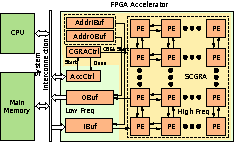
\includegraphics[width=0.99\linewidth]{scgra-accelerator}}
\caption{SCGRA overlay based FPGA accelerator}
\label{fig:scgra-acc}
\end{figure}

\subsection{Loop execution on the accelerator}
\figref{fig:group-dfg} illustrates how the loop is executed 
on the FPGA accelerator. First of all, data flow graph (DFG) is extracted 
from the loop and then it is scheduled on to the SCGRA overlay based FPGA accelerator. 
Depending on how much the loop is unrolled and transformed to DFG, the DFG may be 
executed repeatedly until the end of the original loop. In addition, data transfers for 
multiple executions of the same DFG are batched into groups as shown in \figref{fig:group-dfg}. 
On the one hand, this technique is used to reduce the number of batching, which further 
helps to amortize the initial communication cost. On the other hand, it also 
results in larger on-chip memory overhead. The proposed customization framework 
can be used to make the right design choices to achieve an optimal design. 

\begin{figure}[tb]
\center{\includegraphics[width=0.95\linewidth]{group-dfg}}
\caption{Loop, group and DFG. The loop will be divided into 
groups. Each group will be partially unrolled and the unrolled part will be 
translated to DFG. IO transmission between FPGA and host CPU is performed 
in the granularity of a group.}
\label{fig:group-dfg}
\end{figure}

\subsection{On-chip buffer structure}
On-chip buffer is used to store data transmitted between the FPGA 
accelerator and main memory. (The input and output buffers are quite similar, so 
we just present the input buffer structure here for saving the space.) 
It is usually implemented with block RAM and 
a naive implementation as shown in \figref{fig:naive-implementation} 
provides limited bandwidth to the accelerator which may dramatically 
restrict the performance of the accelerator. A straightforward solution is to 
expose the primitive block RAM ports to the accelerator 
directly as shown in \figref{fig:quick-partition}. However, the bandwidth is 
limited by the number of the primitive block RAM and it works only when 
the data is perfectly placed into different block RAM banks and each port of 
the accelerator accesses exactly the corresponding sub set of the data. In addition, 
we may want to have the input/output data of the same group stored in the input/output 
buffers as mentioned in previous section, while different input/output of the 
DFGs in the same group may have diverse layout pattern. For instance, one DFG 
may load its first input data from partitioned bank 0 while the 
following DFG may have to load its first input data from bank 1. As a result, 
the two DFGs will not be able to reuse the same lock-step computing on the SCGRA overlay. 
Although we may load/store input/output data for each DFG computation, the 
fine-grain data transmission between main memory and FPGA on-chip buffer is extremely 
expensive.

To solve this problem, we have introduced an additional buffering stage and developed 
a scalable on-chip buffer structure as shown in \figref{fig:scalable-partition1} 
and \figref{fig:scalable-partition2}. The first stage is the basic on-chip buffer as 
mentioned in \figref{fig:naive-implementation} and \figref{fig:quick-partition}. It stores 
data of a single transmission between the accelerator and main memory. The additional 
buffer stage stores the input/output of the DFG computation on the CGRA overlay. It ensures the 
input/output data has exactly the same layout for all the DFG computation. Moreover, it can be 
implemented with arbitrary number of FIFOs providing sufficient bandwidth to the accelerator. 

\begin{figure}[tb]
    \centering
	\subfloat[Naive buffer structure]{%
		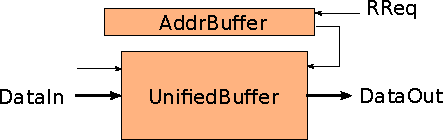
\includegraphics[width=0.3\textwidth]{buffer-type0}
        \label{fig:naive-implementation}
	}\qquad
	\subfloat[Straightforward partitioned buffer structure]{%
		\includegraphics[width=0.35\textwidth]{buffer-type1}
        \label{fig:quick-partition}
	}
    \hfill
	\subfloat[Naive partitioned buffer structure]{%
		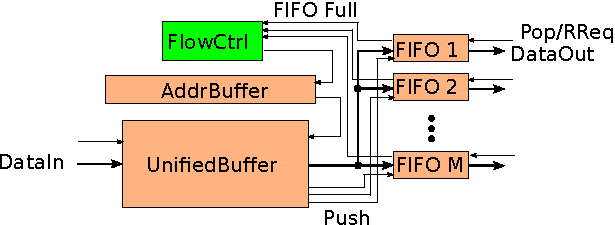
\includegraphics[width=0.45\textwidth]{buffer-type2}
        \label{fig:scalable-partition1}
	}
	\subfloat[Scalable partitioned buffer structure]{%
		\includegraphics[width=0.55\textwidth]{buffer-type3}
        \label{fig:scalable-partition2}
	}
    \caption{On-chip buffer structure}
	\label{fig:on-chip-buffer}
\end{figure}


Although the additional buffer stage makes the computation data path even 
longer, data movement between the first buffer stage and the second buffer 
stage in input/output buffer and the DFG computing in the same group can 
be pipelined as illustrated in \figref{fig:buffer-pipelining}. 
As long as the FIFOs are still available, FlowCtrl will keep the 
first stage buffer sending data to the second buffer stage with the 
pre-scheduled order which is obtained from the CGRA overlay scheduling 
and stored in the AddrBuffer. When the FIFOs have all the input for a 
single DFG execution, FlowCtrl will start the accelerator. When the 
accelerator completes a DFG computing, it will stop until it is activated 
next time. On the output side, the buffer and the accelerator work similarly.
When the number of DFGs included in a group is big enough and DFG computing 
time is larger than the data movement cost, the cost of the 
additional buffer stages can be ignored. 

To support the pipelining in \figref{fig:buffer-pipelining}, 
the overall FIFO capacity is set to be twice the input/output 
of a single DFG. When the time consumed for data movement between 
the two buffer stages is shorter than the DFG computing time, 
\figref{fig:scalable-partition1} can be used. Or else, we may 
make use of all the potential bandwidth in the first buffer stage using 
the buffer in \figref{fig:scalable-partition2}. 

\begin{figure}[tb]
\center{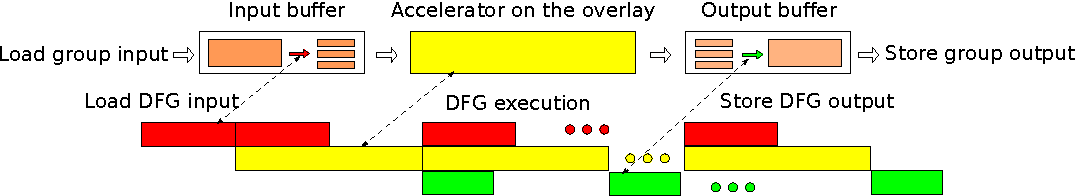
\includegraphics[width=0.9\linewidth]{buffer-pipelining}}
\caption{Pipelined execution on the CGRA overlay}
\label{fig:buffer-pipelining}
\end{figure}


